\documentclass{beamer}


\usepackage{amssymb,amsmath}
\usepackage{graphicx}
\usepackage{url}
\usepackage{color}
\usepackage{relsize}		% For \smaller
\usepackage{url}			% For \url
\usepackage{epstopdf}	% Included EPS files automatically converted to PDF to include with pdflatex

%For MindMaps
% \usepackage{tikz}%
% \usetikzlibrary{mindmap,trees,arrows}%

%%% Color Definitions %%%%%%%%%%%%%%%%%%%%%%%%%%%%%%%%%%%%%%%%%%%%%%%%%%%%%%%%%
%\definecolor{bordercol}{RGB}{40,40,40}
%\definecolor{headercol1}{RGB}{186,215,230}
%\definecolor{headercol2}{RGB}{80,80,80}
%\definecolor{headerfontcol}{RGB}{0,0,0}
%\definecolor{boxcolor}{RGB}{186,215,230}

%%% Save space in lists. Use this after the opening of the list %%%%%%%%%%%%%%%%
%\newcommand{\compresslist}{
%	\setlength{\itemsep}{1pt}
%	\setlength{\parskip}{0pt}
%	\setlength{\parsep}{0pt}
%}

%\setbeameroption{show notes on top}

% You should run 'pdflatex' TWICE, because of TOC issues.

% Rename this file.  A common temptation for first-time slide makers
% is to name it something like ``my_talk.tex'' or
% ``john_doe_talk.tex'' or even ``discrete_math_seminar_talk.tex''.
% You really won't like any of these titles the second time you give a
% talk.  Try naming your tex file something more descriptive, like
% ``riemann_hypothesis_short_proof_talk.tex''.  Even better (in case
% you recycle 99% of a talk, but still want to change a little, and
% retain copies of each), how about
% ``riemann_hypothesis_short_proof_MIT-Colloquium.2000-01-01.tex''?

\mode<presentation>
{
  % A tip: pick a theme you like first, and THEN modify the color theme, and then add math content.
  % Warsaw is the theme selected by default in Beamer's installation sample files.

  %%%%%%%%%%%%%%%%%%%%%%%%%%%% THEME
  %\usetheme{AnnArbor}
  %\usetheme{Antibes}
  %\usetheme{Bergen}
  %\usetheme{Berkeley}		% bem bacana - menu esquerdo
  %\usetheme{Berlin}
  %\usetheme{Boadilla}
  %\usetheme{boxes}
  %\usetheme{CambridgeUS}		% bem bacana - menu superior
  %\usetheme{Copenhagen}
  %\usetheme{Darmstadt}
  %\usetheme{default}
  %\usetheme{Dresden}
  \usetheme{Frankfurt}
  %\usetheme{Goettingen}
  %\usetheme{Hannover}		% bem bacana - menu esquerdo
  %\usetheme{Ilmenau}
  %\usetheme{JuanLesPins}
  %\usetheme{Luebeck}
  %\usetheme{Madrid}		%bacana
  %\usetheme{Malmoe}
  %\usetheme{Marburg}		% bem bacana - menu direito
  %\usetheme{Montpellier}
  %\usetheme{PaloAlto}		% bem bacana - menu esquerdo
  %\usetheme{Pittsburgh}
  %\usetheme{Rochester}		%bacana
  %\usetheme{Singapore}
  %\usetheme{Szeged}
  %\usetheme{Warsaw}

  %%%%%%%%%%%%%%%%%%%%%%%%%%%% COLOR THEME
  %\usecolortheme{albatross}		% azul escuro, massa
  %\usecolortheme{beetle}		% cinza, menu azul
  %\usecolortheme{crane}		% branco e amarelo, massa
  \usecolortheme{default}		% branco, azul clarinho
  %\usecolortheme{dolphin}		% azul e branco, legal
  %\usecolortheme{dove}			% cinza e branco, feio
  %\usecolortheme{fly}			% todo cinza, horrível
  %\usecolortheme{lily}			% parece o default
  %\usecolortheme{orchid}		% azul e branco, ok
  %\usecolortheme{rose}			% branco e violeta-claro, bonito
  %\usecolortheme{seagull}		% cinza, feio
  %\usecolortheme{seahorse}		% nhé, meio feio
  %\usecolortheme{sidebartab}		% Azul, branco, destaque na tab, interessante
  %\usecolortheme{structure}		% bichado
  %\usecolortheme{whale}		% Azul e branco, bem bonito

  %%%%%%%%%%%%%%%%%%%%%%%%%%%% OUTER THEME
  \useoutertheme{default}
  %\useoutertheme{infolines}
  %\useoutertheme{miniframes}
  %\useoutertheme{shadow}
  %\useoutertheme{sidebar}
  %\useoutertheme{smoothbars}
  %\useoutertheme{smoothtree}
  %\useoutertheme{split}
  %\useoutertheme{tree}

  %%%%%%%%%%%%%%%%%%%%%%%%%%%% INNER THEME
  \useinnertheme{circles}
  %\useinnertheme{default}
  %\useinnertheme{inmargin}
  %\useinnertheme{rectangles}
  %\useinnertheme{rounded}

  %%%%%%%%%%%%%%%%%%%%%%%%%%%%%%%%%%%

  \setbeamercovered{invisible} % or whatever (possibly just delete it)
  % To change behavior of \uncover from graying out to totally
  % invisible, can change \setbeamercovered to invisible instead of
  % transparent. apparently there are also 'dynamic' modes that make
  % the amount of graying depend on how long it'll take until the
  % thing is uncovered.

}


% Get rid of nav bar
\beamertemplatenavigationsymbolsempty

% Use short top
%\usepackage[headheight=12pt,footheight=12pt]{beamerthemeboxes}
%\addheadboxtemplate{\color{black}}{
%\hskip0.5cm
%\color{white}
%\insertshortauthor \ \ \ \ 
%\insertframenumber \ \ \ \ \ \ \ 
%\insertsection \ \ \ \ \ \ \ \ \ \ \ \ \ \ \ \ \  \insertsubsection
%\hskip0.5cm}
%\addheadboxtemplate{\color{black}}{
%\color{white}
%\ \ \ \ 
%\insertsection
%}
%\addheadboxtemplate{\color{black}}{
%\color{white}
%\ \ \ \ 
%\insertsubsection
%}

% Insert frame number at bottom of the page.
% \usefoottemplate{\hfil\tiny{\color{black!90}\insertframenumber}} 

\usepackage[english]{babel}
\usepackage[latin1]{inputenc}
\usepackage{subfigure}

\usepackage{times}
\usepackage[T1]{fontenc}


\title[GB21802]{GB21802 - Programming Challenges}
\subtitle[]{Week 0B - Solving Problems}
\author[Claus Aranha]{Claus Aranha\\{\footnotesize caranha\@@cs.tsukuba.ac.jp}}
\institute{Department of Computer Science}
\date{2016/4/15\\{\smaller(last updated: \today)}}

\begin{document}

%% TODO: Add coding examples for each of the hints in this chapter
%% TODO: Add some optional, additional post-hoc problems

\section{Introduction}
\subsection{Class Outline}

\begin{frame}
\maketitle
\end{frame}

\begin{frame}
  \frametitle{Survey Results (Sunday)}

  About 15 respondents:
  \begin{itemize}
  \item Students: Regular: 40\%, Tech School: 40\%, Intl: 20\%
  \item Contest Experience: 10\%
  \item 50\% programs for fun. Only 1 to save the world.
  \item C/C++ are favorite languages, Only 1 likes Python :-(. One
    wants to use Ruby, One wants to use LUA!
  \item Expectations: Programming Contest (1 person), Improving
    programming skill (5 people), Worried about English: 2 People;
  \end{itemize}

  \vfill
  
  \begin{alertblock}{UVA Username}
    Currently, \alert{24 out of 30} people sent me their username.\\
    Don't forget to submit your UVA username!
  \end{alertblock}
\end{frame}

\begin{frame}
  \frametitle{Submission Results (Sunday)}

  \begin{itemize}
  \item Division of Nlogonia: 7 Tried, 6 Succeeded
  \item Cancer or Scorpio: 4 tried, 4 succeeded
  \item 3n+1 Problem: 5 tried, 4 suceeded
  \item Request for Proposal: 2 tried, 2 succeeded
  \end{itemize}

  \vfill

  \begin{center}
    Time to make questions about the problems!
  \end{center}
\end{frame}

\begin{frame}
  \frametitle{Today's Class: Solving Problems}
  \begin{block}{}
    Hints and ideas on how to solve programming challenges
  \end{block}

  \bigskip

  \begin{itemize}
  \item Reading Problems
  \item Considerations when programming
  \item Input/Output
  \item Debugging
  \item Types of Problems
  \end{itemize}
\end{frame}

\section{How to Solve Problems}
\subsection{Programming Challenge Workflow}
\begin{frame}
  \frametitle{A Programming Challenge Workflow}

  \begin{center}
    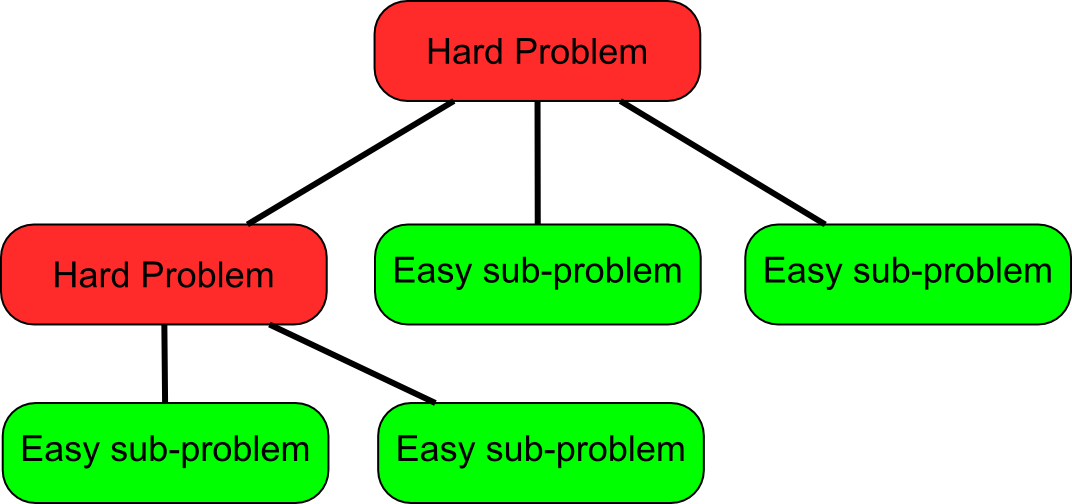
\includegraphics[width=0.5\textwidth]{../img/breakingtheproblem}
  \end{center}

  First trick of solving a hard problem: break it into simpler ones:
  
  {\smaller
  \begin{itemize}
  \item Task 1: Understand the problem description;
  \item Task 2: Understand the input/output;
  \item Task 3: Choose the Algorithm;
  \item Task 4: Write the Code;
  \item Task 5: Test the program on example data until it works;
  \item Task 6: Test the program on hidden data;
  \end{itemize}}
\end{frame}

\subsection{Task 1: Reading The Problem}
\begin{frame}
  \frametitle{Task 1: Understanding the Problem Description}

  Program Challenge descriptions can be hard to understand sometimes:

  \bigskip

  \begin{itemize}
    \item Easy problems usually have extra ``flavor'' text;
    \item Problems with little text are usually harder;
  \end{itemize}

  \bigskip

  Of course, \alert{there are always exceptions!}
\end{frame}

\begin{frame}
  \frametitle{Extreme example: UVA 1124, Celebrity Jeopardy}
  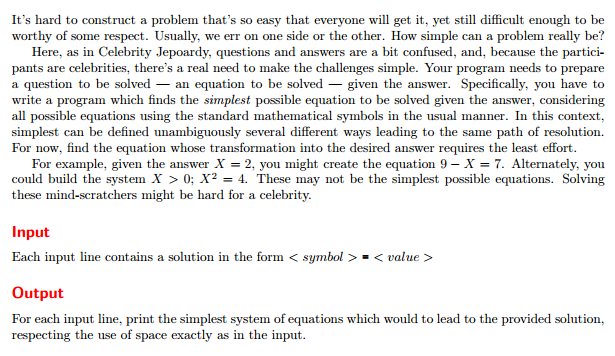
\includegraphics[width=0.9\textwidth]{../img/celebrityjeopardy}

  \hrulefill\\
  \alert{Real Problem:}
  Copy the input into the output.
\end{frame}

\begin{frame}
  \frametitle{Hints for reading text}
  
  \begin{columns}
    \column{0.7\textwidth}
    \begin{itemize}
    \item Read the \structure{Input/Output} sections first, to know
      the \structure{important keywords of a problem};
    \item Read the problem one time, and mark keywords;
    \item Read the problem a second time, and cut phrases that are not
      important;
    \item For harder problem descriptions, copy the important
      information to another file.
    \end{itemize}
    \column{0.3\textwidth}
    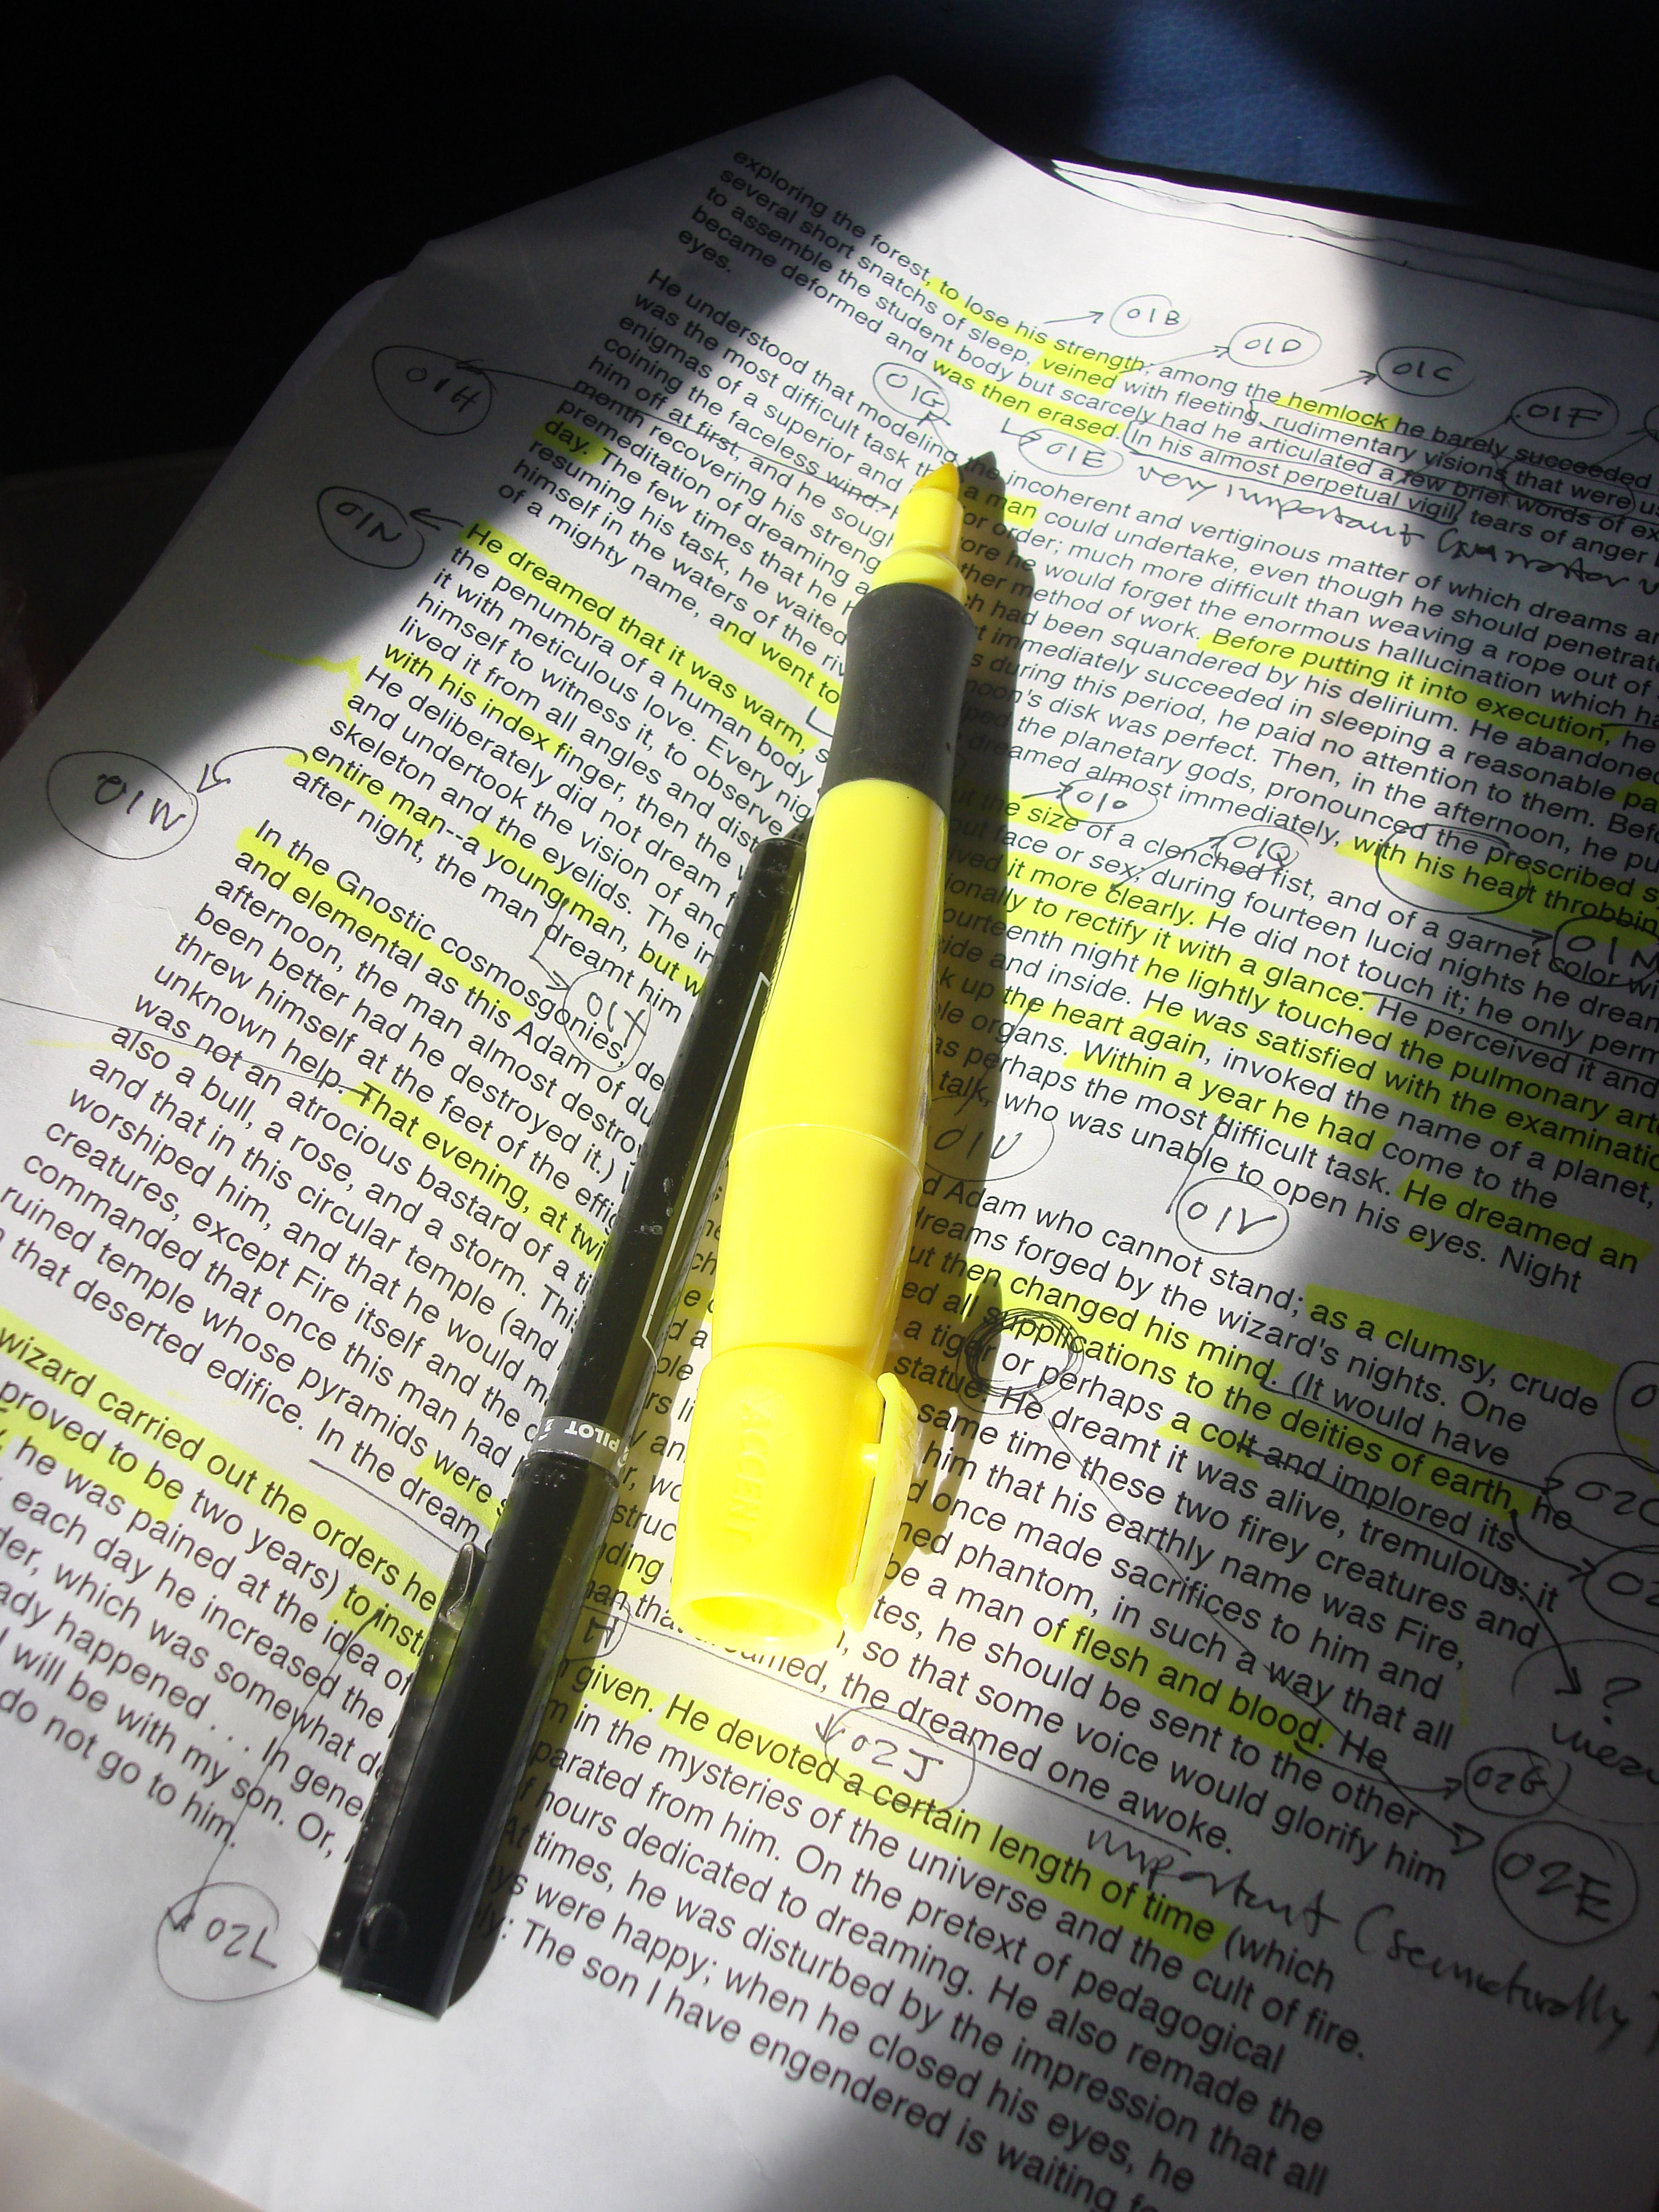
\includegraphics[width=\textwidth]{../img/textmarker}
  \end{columns}

  \vfill

  \hrulefill\\
  \hfill {\tiny Image by Guido ``random'' Alvarez, released as CC-BY-2.0}

\end{frame}

\subsection{Task 2: Understanding the Input/Output}

\begin{frame}
  \frametitle{Understanding the Input}

  Checklist of things we want to learn from the input:
  \smallskip

  \begin{itemize}
  \item Problem Size
  \item Input Format
  \end{itemize}
\end{frame}

\begin{frame}
  \frametitle{Input Size} 
  \structure{Input Size} might be the most
  important information in the text. It will 
  strongly influence your choice of algorithms.

  \begin{block}{Keep in Mind!}
    \begin{itemize}
    \item Most problems have time limits around 1 -- 3 seconds
    \item Around 10.000.000 calculations per second
    \item Don't forget multiplicative effects!
    \end{itemize}
  \end{block}
\end{frame}

\begin{frame}
  \frametitle{Input Size -- Examples}

  \begin{block}{n $<$ 24}
    Exponential algorithms will work (O($2^n$)).\\
    Or sometimes you can just calculate all solutions.
  \end{block}

  \begin{block}{n = 500}
    Cubic algorithms don't work anymore (O($n^3$) = 125.000.000)\\
    Maybe O($n^2\text{log}n$) will still work.
  \end{block}

  \begin{block}{n = 10.000}
    A square algorithm (O($n^2$)) might still work.\\
    But beware any big constants!
  \end{block}

  \begin{block}{n = 1.000.000}
    O($n$log$n$) = 13.000.000\\
    We might need a linear algorithm!
  \end{block}
\end{frame}

\begin{frame}[fragile,singleslide]
  \frametitle{Input Types (1)}
  \begin{block}{N lines}
    The input tells the number of lines to be read in advance.\\
    \structure{Example:} 11947 -- Cancer or Scorpio
  \end{block}

{\smaller 
\begin{verbatim}
#include <iostream>
using namespace std;

int main()
{
    int n;
    string input;
    
    cin >> n;
    for (int i = 0; i < n; i++)
    {
        cin >> input;
        // Do your work!
    }    
}
\end{verbatim}}

\end{frame}

\begin{frame}[fragile,singleslide]
  \frametitle{Input Types (2)}
  \begin{block}{Conditional Ending}
    The input starts with a condition (number of elements, etc), and 
    a special case indicates the end of the input.\\
    \structure{Example:} 10141 -- Request for Proposal
  \end{block}

{\smaller
\begin{verbatim}
int main()
{
   cin >> n >> p;
   cin.ignore(1000, '\n'); 
   // throws away the \n for a future getline
   while (n!=0 || p!=0)
   {
       // do your work!
       cin >> n >> p;               
       cin.ignore(1000, '\n');
   }
}
\end{verbatim}}
\end{frame}

\begin{frame}[fragile,singleslide]
  \frametitle{Input Types (3)}
  \begin{block}{End of File}
    The input goes on until the end of the file. No explicit
    terminating value.\\
    \structure{Example:} 100 -- The N+1 Problem
  \end{block}
{\smaller
\begin{verbatim}
#include<string>
int main()
{
    string n;
    while (getline(cin,n))
    {
        // Solving your problem
    }
}
\end{verbatim}
}
\end{frame}

\begin{frame}
  \frametitle{Reading the Output -- Correctness}

  The UVA judge will evaluate your code based on a simple \emph{diff}. 
  Be \alert{very careful} to write your output exactly like stated.

  \vfill

  \begin{columns}
    \column{0.2\textwidth}
    
\includegraphics[width=1\textwidth]{../img/angryclient}
    \column{0.7\textwidth} \emph{The Judge is like an angry client. It
      wants the output EXACTLY how it stated.}
  \end{columns}
\end{frame}

\begin{frame}
  \frametitle{Easy to Miss errors in the output}

  
\includegraphics[width=0.15\textwidth]{../img/angryclient}
  \begin{itemize}
  \item Are the words uppercase, or lower case? (Case \structure{or} case)
  \item Are there any mistakes in the words? (case \structure{or} caes)
  \item Singular or plural? (1 hours \structure{or} 1 hour)
  \item What is the precision of floating numbers? (3.051 \structure{or} 3.05)
  \item Do you round up or round down? (3.62 $\rightarrow$ 3 \structure{or} 4)
  \end{itemize}
\end{frame}

\begin{frame}
  \frametitle{Other things to pay attention in the output}
  
\includegraphics[width=0.15\textwidth]{../img/angryclient}
  \begin{itemize}
  \item Do you need to output the \structure{entire solution} or just
    the \structure{solution cost}?
  \item Are there multiple solutions? Which one must you output?
  \end{itemize}
\end{frame}

\begin{frame}
  \frametitle{Reading the problem: Identify Traps!}
  Be very careful to limits \alert{not stated} in the problem:
  \begin{itemize}
    \item \structure{3n+1}: The input gives $i$ and $j$, but there is
      no guarantee that $i$ > $j$.
    \item \structure{Cancer or Scorpio}: You have to take leap years
      into account.
  \end{itemize}

  \vfill

  \hfill 
\includegraphics[width=0.25\textwidth]{../img/trap}
\end{frame}

\begin{frame}
  \frametitle{Reading the problem: Identify Traps!}
  Other common traps:
  \begin{itemize}
  \item Negative numbers, No maximum limit;
  \item Repeated Numbers;
  \item (in graphs) circular edges, duplicate edges;
  \item (in geometry) duplicate points;
  \item (in paths) two paths with same cost, no solutions;
  \end{itemize}

  \hfill 
\includegraphics[width=0.25\textwidth]{../img/trap}
\end{frame}

\subsection{Task 3: Choosing the algorithm}

\begin{frame}
  \frametitle{Task 3: Choosing the algorithm}
  \begin{block}{3.1 What type of problem it is?}
    \begin{itemize}
    \item Full Search: Tests all possible solutions;
    \item Greedy: Break the solution, and try each best subsolution;
    \item Simulation: Execute a series of steps, record the results;
    \item Dynamic Programming: Table of partial solutions;
    \item Counting: Calculate the number of possible solutions;
    \item Ad-hoc: No fixed category;
    \item And many others;
    \end{itemize}
  \end{block}

  \bigskip

  We will see examples of each category during the course.
\end{frame}

\begin{frame}
  \frametitle{Task 3: Choosing the algorithm}
  Basic considerations for recursive and iterative algorithms:

  \begin{itemize}
  \item An algorithm with k-nested loops of about n iterations each
    has O(nk) complexity;
  \item A recursive algorithm with b recursive calls per level, and L
    levels, it should have O(bL) complexity;
  \item This complexity can be reduced with pruning;
  \item An algorithm processing a $n*n$ matrix in O(k) per cell runs
    in $O(kn^2)$ time. 
  \end{itemize}
\end{frame}

\begin{frame}
  \frametitle{Task 3: Choosing the algorithm}
  
  We will talk about data structures next class, but see this example:

  \begin{block}{3.2: What data structure should we use?}
    Number of Solutions for the 8-queen problem:
    \begin{itemize}
    \item 8x8 matrix, with 1 for each queen: 64*63*62... = 1.78e+14
    \item 1 queen per column: 8*8*8*... = 1.67+e8
    \item 1 queen per column/row: 8*7*6... = 40320
    \end{itemize}

    \bigskip

    You can remove even more solutions by pruning simetries.
  \end{block}
\end{frame}

\subsection{Task 4: Coding}


\begin{frame}
  \frametitle{Task 4: Coding} 

  \structure{Programmer Efficiency}: Different from time efficiency,
  programmer efficiency measures how much a code taxes your mind.

  \begin{itemize}
  \item Understandable program! (not a lot of boiler plate)
  \item Simpler structures to avoid hard bugs (avoid memory allocation)
  \item Using ``Good Enough'' algorithms (avoid overcomplexity)
  \item Use standard libraries and Macros
  \end{itemize}


  \begin{exampleblock}{Hint: Library File}
    Create an extra file with macros, functions and structures you use
    often. Add to this file as you learn new techniques. 
  \end{exampleblock}
\end{frame}

\begin{frame}
  \frametitle{Task 4: Coding}
  \begin{block}{Hint 1: Use paper}
    \begin{itemize}
    \item Think first
    \item Code second
    \end{itemize}
  \end{block}

  \begin{exampleblock}{Hint 2: Type fast}
    Practice typing in one of many online typing challenges.
    \begin{itemize}
    \item \url{www.typingtest.com}
    \item \url{https://typing.io} -- for programmers!
    \end{itemize}    
  \end{exampleblock}
\end{frame}

\subsection{Testing}
\begin{frame}
  \frametitle{Test and Hidden Data}

  The problem description in UVA shows the \structure{Example
    Data}. But the actual judge also uses \alert{Hidden Data}. 

  \begin{columns}
    \column{0.45\textwidth}
    \begin{exampleblock}{Example Data}
      \begin{itemize}
      \item Useful to test input/output;
      \item Read the example data to understand the problem;
      \item Minimal condition to say your program work;
      \end{itemize}
    \end{exampleblock}
    \column{0.45\textwidth}
    \begin{alertblock}{Hidden Data}
      \begin{itemize}
      \item Actual judging will happen with different data;
      \item Usually harder and longer data sets;
      \item Including bully and worst cases;
      \end{itemize}
    \end{alertblock}
  \end{columns}
  
  \medskip

  Generate your own set of hidden data before submitting!
\end{frame}

\begin{frame}
  \frametitle{What data to generate?}

  \begin{itemize}
  \item Datas with multiple entries (to check for initialization);
  \item Datas with maximum size (can be trivial cases);
  \item Random data;
  \item Border cases (maximum and minimum values in input range);
  \item Worst cases (depends on the problem);
  \end{itemize}
\end{frame}

\begin{frame}
  \frametitle{The uDebug Website}

  \begin{center}
    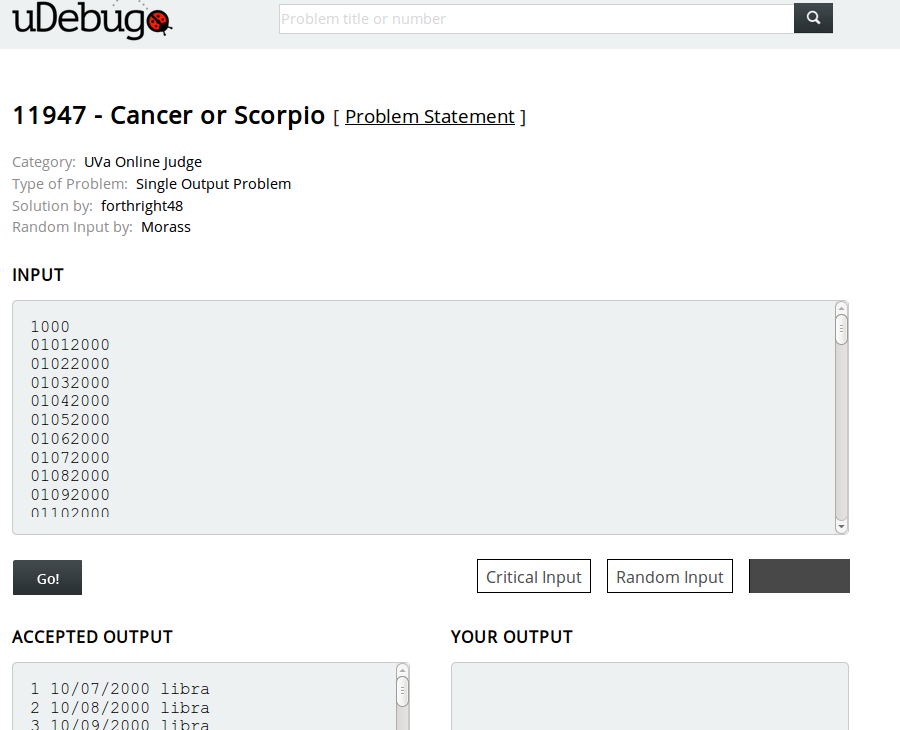
\includegraphics[width=0.8\textwidth]{../img/udebug_big}
  \end{center}
\end{frame}



\section{Conclusion}
\subsection{The End}
\begin{frame}
  \frametitle{To Summarize}
  Mental framework to solve problems:
  \begin{enumerate}
  \item Read the problem carefully to avoid traps;
  \item Think of the algorithm and data structure;
  \item Keep the size of the problem in mind;
  \item Keep your code simple;
  \item Create special test cases;
  \end{enumerate}

  \vfill

  \begin{block}{}
    Now go solve the other problems!
  \end{block}
\end{frame}

\begin{frame} 
  \frametitle{Thanks for Listening!}
  \begin{center}
    Any questions?
  \end{center}
\end{frame}

\begin{frame}
  \frametitle{BONUS I -- The most expensive program ever?}

  \begin{block}{Ackermann's Function}
    \begin{eqnarray*}
      A(m,n) = & n+1 & \text{if } m = 0\\
      & A(m-1,1) & \text{if } m > 0, n = 0\\
      & A(m-1,A(m,n-1)) & \text{if } m > 0, n > 0\\
    \end{eqnarray*}
  \end{block}
  
  \begin{itemize}
    \item $A(0,n) = n+1$
    \item $A(1,n) = n+3$
    \item $A(2,n) = 2n+3$
    \item $A(3,n) = 2^{n+3}-3$ \alert{!}
    \item $A(4,n) = 2^{2^{...^2}}-3$ \alert{!!!} (exponential tower of n+3)
    \item $A(5,n) = $ \alert{!!!!!!!!!!!!}
  \end{itemize}
\end{frame}

\begin{frame}
  \frametitle{BONUS II -- More Info on the ICPC Programming Challenge}
  \begin{itemize}
  \item Application deadline: 06/10 (Fri) -- 3-people team
  \item Internet based contest: 06/24 (Fri) -- At Tsukuba
  \item Webpage: \url{http://icpc.iisf.or.jp/2015-tsukuba/?lang=ja}
  \end{itemize}
  \bigskip

  Ask me for details!
\end{frame}

\end{document}
